\begin{figure}
	
	\floatbox{figure}[\FBwidth]
	{
		\caption{NBER working paper release dates vis-à-vis Journal submission dates}\label{figure8}
	}
	{
		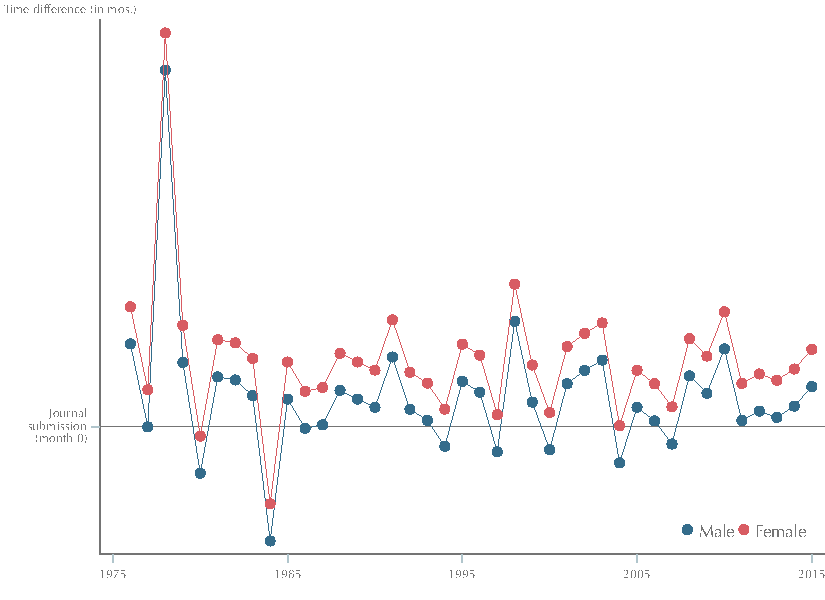
\includegraphics[width=12.3cm]{$HOME/Dropbox/Readability/draft/pdf/figure8.pdf}
		\floatfoot{\tiny \textit{Notes}. Gender differences in the time between the release of a paper as an NBER Working Paper and submission to \textit{Econometrica}. Horizontal grey line denotes that the paper was submitted to \textit{Econometrica} and released as an NBER Working Paper at the same time. Values below this line indicate that papers in a year were, on average, released as an NBER Working Paper before they were submitted to \textit{Econometrica}; values above this line indicate that papers in a year were, on average, submitted first to \textit{Econometrica} and then released as an NBER Working Paper. Points in blue are effect estimated for 100 percent male-authored papers; points in pink are effects estimated for 100 percent female-authored papers.}
	}
\end{figure}